\section{Introduction}
\label{sec:intro}
% Wheat is one of the principal cereal crops, serving as a dietary staple for billions of people worldwide. In order to increase the yield of wheat, the farmers need detailed analysis of wheat plants. With the development of deep learning, using deep neural networks for agricultural image analysis has become the most economical and effective method. In the analysis of wheat plants, wheat organs such as heads, leaves and stems are all of great importance. Therefore, the plant scientists and farmers need a robust model to segment wheat organs from images.

The 7th International Workshop on Machine Learning for Cyber-Agricultural Systems (MLCAS 2025), in conjunction with the Computer Vision in Plant Phenotyping and Agriculture (CVPPA) workshop at International Conference on Computer Vision (ICCV 2025), host a competition called Global Wheat Full Semantic Segmentation (GWFSS). %\footnote{\url{https://www.codabench.org/competitions/5905/}} 
The competition aims to advance pixel-level understanding of wheat plants, \textit{i.e.}, segmenting the full plant components, including four classes of \texttt{leaf}, \texttt{stem}, \texttt{head}, and \texttt{background}, to comprehensively describe plant architecture, health, and development. In this report, we present our winner solution to this competition. % for this task, which contains three stages: 1). first, we train a SOAT semantic segmentation model with limited labeled data; 2). second, we apply the pipeline of semi-supervised learning to learn a robust model; 3). finally, we apply test time scaling during inference.

% 【图】  有监督阶段模型在验证集上的可视化结果（动机）、
\begin{figure}[!t]
    \centering
    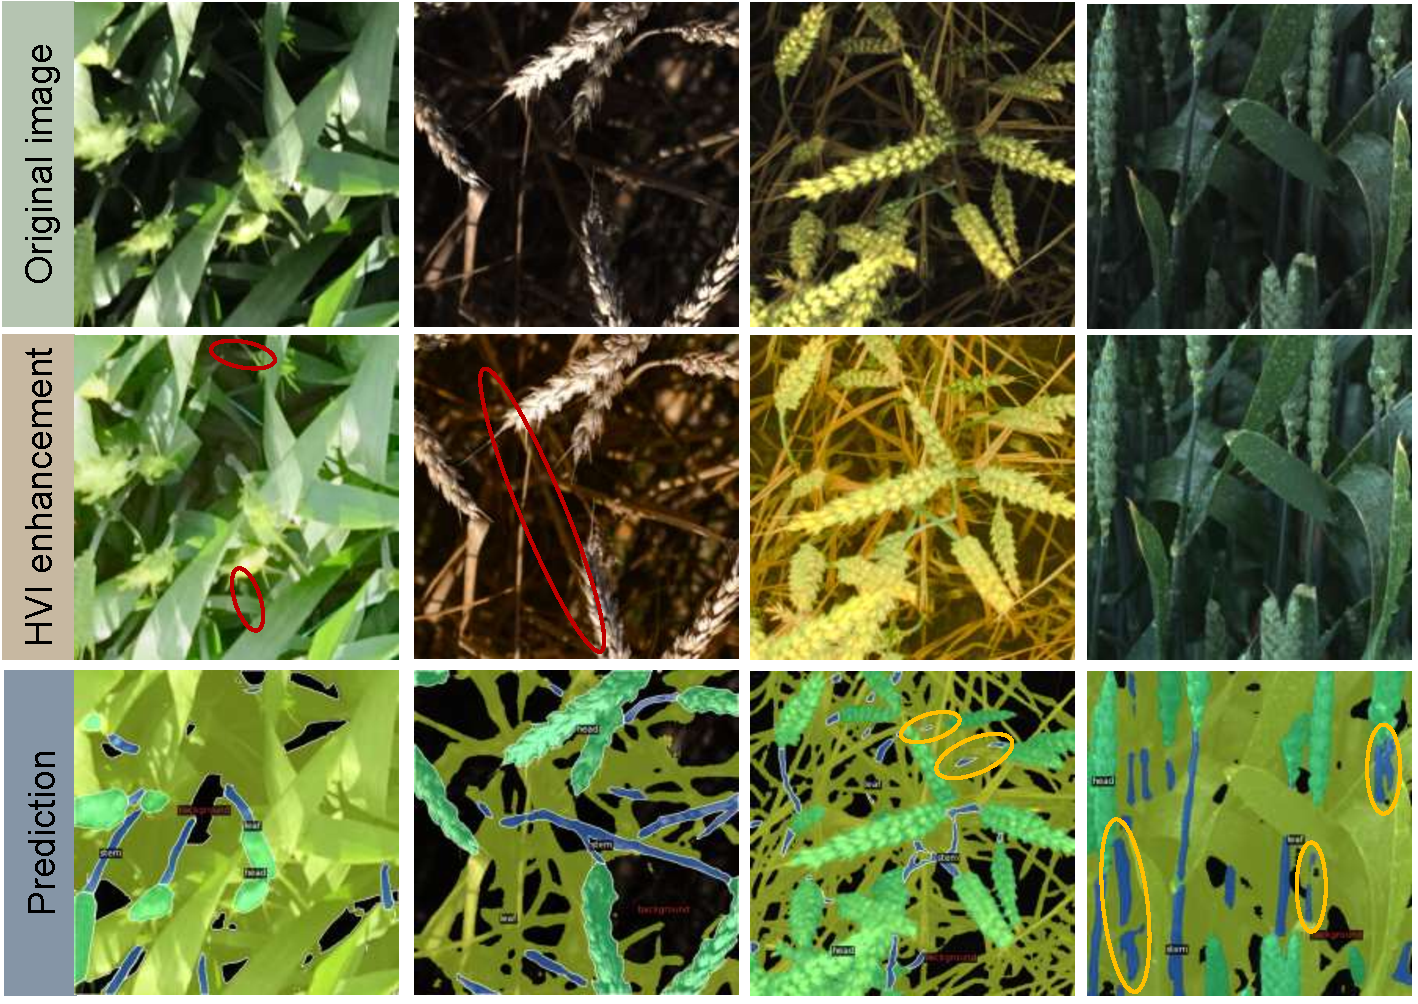
\includegraphics[width=\linewidth]{stage1_vis.pdf}
    \caption{\textbf{Visual inspection of the ViT-Adapter predictions on the GWFSS validation set}. Our intuition tell us that the performance bottleneck seems to lie in the \texttt{stem} class, which not only requires good detail delineation but also needs to tackle the minority of pixel occupancy. Images in the second row are enhanced by the HVI color space~\cite{yan2025hvi} for ease of interpretation. The red circle seems to be stems segmented missed and the yellow one seems to be stems segmented roughly.}
    \label{fig:stage1_vis}
\end{figure}

The competition has two phases. In the development phase (Phase 1), participants can have access to a small subset of fully labeled training data (only $99$ samples) and a large amount of unlabeled data ($64,368$ samples); validation data (only images) are provided for participants to build and iterate their models. In the testing phase (Phase 2), the top 20 participants are invited to generate inference results on the test set using the final model from Phase 1. 
% It is worth noting that there are three main limitations during the development phase
Different from other unconstrained open challenges, there are three rules in this competition: i) only ImageNet-1K pre-trained backbones are allowed to use; ii) only the provided GWFSS training data is allowed to use, and participants cannot use other unlabeled datatsets for pre-training; iii) manual labeling or annotation is strictly prohibited. 

To quickly gain a % comprehensive understanding
first impression of the visual challenges of this task, we trained a state-of-the-art ViT-Adapter with the Mask2Former head using the labeled training data. % This model achieved a score of 0.7284 on the development leaderboard, and 
Some visualizations on the validation set are shown in the Fig.~\ref{fig:stage1_vis}. Due the significant illumination variations, we resort to a recent learnable HVI color space~\cite{yan2025hvi} for ease of interpretation of segmentation results. This color space significantly enhances the contrast of low-light regions such as shadows and reveals many missing details. According to Fig.~\ref{fig:stage1_vis}, we have the following observations and insights.

\begin{remark}
    The fine structure of the stem class leads to difficult boundary predictions such that the model needs to enhance detail awareness.
\end{remark}

By observing the patterns of visualization results, we find that % many images were
the \texttt{head}, \texttt{leaf}, and \texttt{background} classes are well segmented in general, while the \texttt{stem} class exhibits a % higher number 
high
degree of % incorrect
fragile predictions. % and omissions. 
We % also evaluated the final 
therefore test the class IoU metric on the training dataset with available ground truths: the \texttt{stem} class only reports $0.69$ mIoU, while the other three classes achieve $0.88$, $0.91$, and $0.90$ for \texttt{background}, \texttt{head}, and \texttt{leaf}, respectively. It seems that the performance bottleneck lies in the \texttt{stem} class. In our view, we believe an effective way to alleviate this bottleneck is to enhance detail awareness of the model. Technically, this amounts to the question on how to improve the quality of high-resolution feature maps. % the model's ability to understand fine details depends on the quality of the high-resolution feature maps. In Mask2Former, the upsampling steps in the decoder all use bilinear interpolation. Replacing them with dynamic upsampling operators might improve the model's ability to capture fine details. 

\begin{remark}
    The model may risk overfitting due to rather limited labeled data such that unlabeled data should be exploited.
\end{remark}
% In this competition, the amount of labeled training data is very limited, 
The labeled training data are limited (only $99$ images are provided), but our baseline model has more than $200$M parameters, which makes it prone to overfitting. Therefore, how to effectively leveraging the unlabeled data seems to be another key to improve model generalization. In open literature, there are two mainstream ways to exploit the unlabeled data: i) resorting to self-supervised learning to pre-train a vision backbone (e.g., MAE~\cite{he2022masked} and DINOv2~\cite{oquab2023dinov2}); ii) leveraging semi-supervised learning to learn a robust model (e.g. Mean Teacher~\cite{tarvainen2017mean}). We will choose one of the two routes. 

\begin{remark}
    The stem class only occupies a small number of pixels such that the model may suffer from class imbalance.
\end{remark}
By analyzing the number of pixel labels of each class in the training dataset, we find that the proportions of \texttt{background}, \texttt{head}, \texttt{stem}, and \texttt{leaf} pixels are $85$ : $27$ : $9$ : $137$, respectively. It seems \textit{the devil is in the detail and minority}: the stem class is not only subtle to segment but also underrepresented in the dataset. % , which results in the model achieving an mIoU of only $0.69$ even on the training set. 
Hence, we believe we also need to address the class imbalance issue and increase the visibility of the \texttt{stem} class during model training. % imTo balance the distribution of each class, we selectively utilize the unlabeled data during the semi-supervised learning. Specifically, instead of using all the unlabeled data, we selected a subset of samples from each domain where the stem class has the highest proportion.

To address the challenges above, we build upon a state-of-the-art segmentation framework ViT-Adapter~\cite{chen2022vision} and present three technical improvements. % In this report, we present our solution. 
Considering that detail delineation is closely related to the quality of high-resolution feature maps, we first incorporate a dynamic upsampling operator SAPA~\cite{lu2022sapa} into the Mask2Former head~\cite{cheng2022masked} to enhance the detail delineation of the model. % Due to the competition's constraints on the pre-trained weights, we selected the BEiT v2 model pretrained on ImageNet-1K. The final model achieves a score of 0.7291 on the leaderboard. 
Second, we apply a semi-supervised learning pipeline with guided distillation~\cite{berrada2024guided} to leverage the unlabeled training set. Note that,   to alleviate the class imbalance and increase the exposure of the \texttt{stem} class, we do not use the entire unlabeled data but carefully choose a small portion of stem-related image data to form a subset (4500 images), filtered by a model trained with labeled training data. % Instead, we first used the model obtained in the first step to infer on the unlabeled data, then calculated the pixel proportion of the stem class in the predictions. For each domain, we selected the top $500$ samples with the highest stem pixel proportion as the final unlabeled data. Based on $99$ labeled images and $4,500$ selected unlabeled images, our model achieved a score of 0.7432 on the leaderboard. 
Finally, we conduct a form of test-time scaling with a \textit{zoom in and segment twice} strategy, which zooms in images to different scales and segment the image of each scale following a sliding-window style inference. This strategy significantly benefits the prediction of the \texttt{stem} class. % during the test time, we scale images to different size and inference on every image using sliding window. After test time scaling, our model achieved a score of 0.7704 on the leaderboard, which is the highest score in the development phase.
Combining the three improvements, our final solution achieves the first place in the competition during both the development phase and the testing phase, reporting $0.77$ and $0.75$ mIoU metric, respectively, outperforming the second place by clear margins. While the three improvements seem simple, we hope our solution can inform the plant phenotyping community that a simple tweak can make a difference if one identifies the bottleneck correctly.